% CVPR 2023 Paper Template
% based on the CVPR template provided by Ming-Ming Cheng (https://github.com/MCG-NKU/CVPR_Template)
% modified and extended by Stefan Roth (stefan.roth@NOSPAMtu-darmstadt.de)

\documentclass[10pt,twocolumn,letterpaper]{article}

%%%%%%%%% PAPER TYPE  - PLEASE UPDATE FOR FINAL VERSION
\usepackage[final]{cvpr}      % To produce the REVIEW version
%\usepackage{cvpr}              % To produce the CAMERA-READY version
%\usepackage[pagenumbers]{cvpr} % To force page numbers, e.g. for an arXiv version

% Include other packages here, before hyperref.
\usepackage{graphicx}
\usepackage{amsmath}
\usepackage{amssymb}
\usepackage{booktabs}


% It is strongly recommended to use hyperref, especially for the review version.
% hyperref with option pagebackref eases the reviewers' job.
% Please disable hyperref *only* if you encounter grave issues, e.g. with the
% file validation for the camera-ready version.
%
% If you comment hyperref and then uncomment it, you should delete
% ReviewTempalte.aux before re-running LaTeX.
% (Or just hit 'q' on the first LaTeX run, let it finish, and you
%  should be clear).
\usepackage[pagebackref,breaklinks,colorlinks]{hyperref}


% Support for easy cross-referencing
\usepackage[capitalize]{cleveref}
\crefname{section}{Sec.}{Secs.}
\Crefname{section}{Section}{Sections}
\Crefname{table}{Table}{Tables}
\crefname{table}{Tab.}{Tabs.}


%%%%%%%%% PAPER ID  - PLEASE UPDATE
\def\cvprPaperID{*****} % *** Enter the CVPR Paper ID here
\def\confName{CVPR}
\def\confYear{2022}


\begin{document}

%%%%%%%%% TITLE - PLEASE UPDATE
\title{Applying Pose Estimation to Predict the Outcome of Basketball Shots}

\author{Laith Altarabishi\\
University of Texas at Austin\\
{\tt\small laithaustin@utexas.edu}
% For a paper whose authors are all at the same institution,
% omit the following lines up until the closing ``}''.
% Additional authors and addresses can be added with ``\and'',
% just like the second author.
% To save space, use either the email address or home page, not both
\and
Sidharth Babu\\
University of Texas at Austin\\
{\tt\small sidharth.n.babu@utexas.edu}
\and
Afnan Mir \\
University of Texas at Austin\\
{\tt\small afnanmir@utexas.edu}
\and
Zayam Tariq \\
University of Texas at Austin\\
{\tt\small zayamtariq@utexas.edu}
}
\maketitle

%%%%%%%%% ABSTRACT
\begin{abstract}
  In this report, we present an end-to-end pipeline that includes a pose estimator as well as 
  a classification model that can effectively predict the outcome of a free throw. Our training data was
  self-generated by recording hundreds of clips of our test subject shooting free throws of various forms
  and recording the outcome. We explore different ways to generate feature vectors for inputs to our model as 
  well as multiple classification models to produce the best performing pipeline.
\end{abstract}


%%%%%%%%% BODY TEXT
\section{Introduction}
\label{sec:intro}

In basketball, the ability of a player to effectively shoot the basketball typically comes down to the player’s shooting form. While the form of the best shooters tend to look different, they all typically use the same fundamentals. In our project, we will attempt to capture these fundamental aspects of a player’s shooting form and attempt to predict the outcome of a shot using these features. Research has been done on extracting features from a player’s movement to classify the action a player is performing (shooting, dribbling, etc.) \cite{Basketball}, but we would like to focus our energy on feature extraction from the shooting motion using pose estimation \cite{OpenPose}, object detection \cite{YOLO}, and possibly other methods to extract feature descriptors of a shot and attempt to identify it as a make or a miss.\\
\indent This problem is a particularly nontrivial application of pose estimation for two main reasons. The first being that there are multiple stages to
a basketball shot that need to be taken into account. From dipping the ball to waist level, to the motion of bringing the ball to eye level, to releasing the ball, each
plays a significant role in the outcome of a shot, so each stage needs to be taken into account. The second reason is the variability of the average shot. It can be argued that no two shots will ever be identical due to the imperfect nature of humans.
Therefore, it is necessary for our feature representation of a shot to be invariant towards miniscule changes
in shot form and focus more on fundamental differences.
%-------------------------------------------------------------------------
%------------------------------------------------------------------------
\section{Related Works}
\label{sec:formatting}

%-------------------------------------------------------------------------
\subsection{Pose Estimation}

Pose Estimation is a critical topic in computer vision that will intersect with our goal of trying to accurately capture the motion and actions of a person taking a shot in basketball. Pose estimation, in the context of 2D videos of humans, is the problem of localizing anatomical keypoints or joints in a frame by frame video or image \cite{OpenPose}. To fulfill our goal of predicting the outcome of a basketball shot, it will be critical to assess the form of a player who's taking a shot - where form can be decomposed into various classifications of joints in space. Pose estimation methods can be categorized into bottom-up or top-down methodologies. Bottom-up methodologies start by estimating keypoints and body joints first, and then these points are clustered to form poses. In contrast, 
top-down methodologies of pose estimation first run a person detector before decomposing each person into their respective body joints within detected bounding boxes \cite{Viso2}. Computational complexity is a major consideration for landmark pose estimation algorithms, and modern SOTA pose estimation algorithms deploy deep learning and CNNs to improve compuational overhead and speed \cite{OpenPose}. We list some examples of prevalent and SOTA pose estimation models that have been employed and researched below.
%
\begin{quotation}
  OpenPose: The first multi-person realtime 2D pose estimation system that uses a bottom-up approach that implements nonparametric representation to associate human keypoints and body parts with an individual in an image \cite{OpenPose}. \\
  \newline
  \indent DeepPose: SOTA pose estimation method that uses DNNs to classify human body joints through the usage of cascading DNN regressors that produce high precision pose estimates \cite{DeepPos}. \\
  \newline
  \indent AlphaPose: Multi-person SOTA realtime pose estimation system that outperforms OpenPose in AP score and has a high mAP score \cite{Alpha}. \\
  \newline
  \indent DeepCut: Proposes an approach to solving issues in both pose estimation and detection by using a partitioning and labeling formulation of a set of CNN part detectors \cite{DeepCut}.
\end{quotation}

Pose estimation attempts to detect the location of 17 keypoints on a human body, as seen in Figure \ref{fig:pose}. These keypoints include key joints such as
the knee, elbow, shoulder, and wrist, which can be vital in determining the form of a free throw.
\begin{figure}[h]
  \centering
  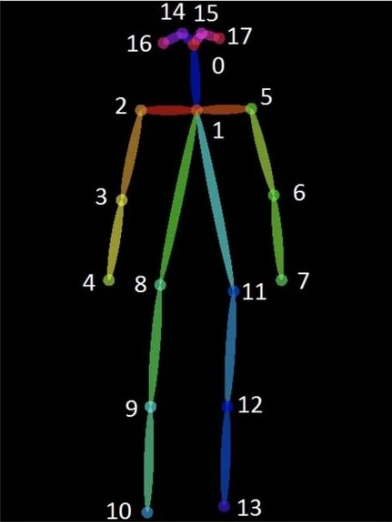
\includegraphics[width=0.25\textwidth]{imgs/openpose.png}
  \caption{Pose estimation keypoints}
  \label{fig:pose}
\end{figure}
%
 
%-------------------------------------------------------------------------
\subsection{Basketball and Pose Estimation}

The application of pose estimation in basketball is not a new concept. Collecting and analyzing basketball player's
posture data is an important facet of the scientific basketball community in order to help maximize training outputs.
For example, pose estimation was used in combination with classification models to predict the action a player is performing
in a video \cite{Basketball}. This is fairly similar to our project because it attempts to create feature vectors in video frames
using pose estimation to encode data about the motion of a player and use these features to make a prediction. However, our project
solely focuses on the motion of a player's shooting form and predicting the outcome of the shot.

%

%-------------------------------------------------------------------------
\subsection{Object Detection}

Our project will hope to capture and detect objects in high frame-rate video, with minimal computational overhead so that we are able to best assess the keypoints/human joints of our basketball shooters. 
In recent years, object detection algorithms have evolved greatly and most SOTA models today utilize deep learning to provide more robust results \cite{Viso}. There are many pre-existing SOTA object detection methods that have been utilized in the context of pose estimation methods and regression issues, and the following works are examples of some of them.

\begin{quotation}
  YOLO: Single stage object detection algorithm that frames detection as a regression problem to spatially seperated bounding boxes and associated class probabilities \cite{YOLO}.\\
  \newline
  \indent Mask R-CNN: Two-stage object detection algorithm that detects objects in an image while creating high-quality segmentation masks for each instance \cite{PatternRec}.\\
  \newline
  \indent Feature Pyramid Networks: Two-stage object detection algorithm that uses the multi-scale, pyramidial hierarchy of deep convolutional networks to create feature pyramids \cite{FeaturePyr}. \\
\end{quotation}

%------------------------------------------------------------------------
\section{Methodology}
\subsection{General Overview}
% We will have a camera taking in video input of a player shooting the basketball, potentially from two different angles.
% One angle would be a side view of the shooter that can capture the relative positions of the shooter and the hoop, and the other
% would be a head-on view of the of the shooter to capture the full pose estimation of the shooter.

% In the background, we will have our pose estimation algorithm running to capture the pose estimation of the shooter which will be used
% to make our predictions. Additionally, we will potentially be retrieving other data to create our feature vector, including the angle relationship
% between the shooter and the hoop, and the speed of the shot. We will be attempting to capture the pose estimation at multiple stages of the
% shot, as each stage can have a significant impact on the outcome of the shot. We will then take this feature vector and put it through a classification model.
% We will perform binary classification and predict whether a shot will go in or not.
The high-level overview of our end-to-end pipeline is shown in Figure \ref{fig:flowchart}. We start off by capturing clips of a test subject shooting a free throw. This will be our 
original data. We first want to downsample the video as we assume that many of the frames will be redundant and take up unnecessary computation time. After this, we perform pose estimation
on all the frames of each video to get the keypoints of our test subject for each video clip. Using the pose estimation data, we perform
feature extraction to generate feature vectors for each video clip according to some convention. This will be elaborated on in a later section. 

These feature vectors will be the training and testing data that we use for our classification model. We will want to split this data into training
and testing sets. We will train our classification model on the training set and generate predictions using our testing set.
\begin{figure}[h]
  \centering
  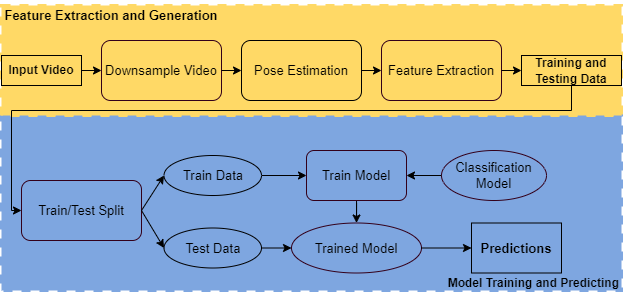
\includegraphics[width=0.45\textwidth]{imgs/cv_pipeline_real.png}
  \caption{Overview of Pipeline}
  \label{fig:flowchart}
\end{figure}

\subsection{Data Collection}
To fit the scope of our project, we wanted the shot data be as controlled as possible to prevent unwanted variations
in our data. To do this, we collected our own data, where we had our test subject always shoot from the free throw line
and had a camera in a fixed position in front of the test subject to capture their form. The set up can be seen in Figure \ref{fig:ft_data}.
We genereated approxiamately 300 clips of our test subject shooting free throws. Additionally, for this project, we wanted to detect major changes
in shooting forms that could affect the outcome of a shot. Therefore, our test subject shot some of their shots as he normally would, with the intent
of making it, and some of their shots with purposefully bad form, with the intent of missing. We had a relatively even split of these two types of shots. 

\begin{figure}
  \centering
  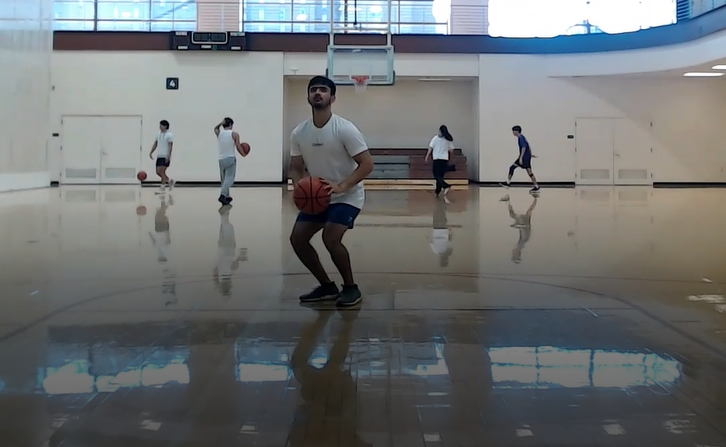
\includegraphics[width=0.45\textwidth]{imgs/data_collection.png}
  \caption{Free Throw}
  \label{fig:ft_data}
\end{figure}

\subsection{Pose Estimation}
As far as pose estimation goes, it seems that a bottom up approach to pose estimation will be the best approach for our use case, as the bottom up approach is the
current state of the art when it comes to pose estimation and is computationally less expensive \cite{Datagen}. There are a few state of the art bottom up pose estimation libraries that we could potentially use. These
libraries include OpenPose, AlphaPose, DeepCut, and MoveNet. We will test these libraries on their latency and accuracy. With a basketball shot, we want minimum latency
as well as an ability to run at a high frames per second (FPS) quantity. We will use these metrics as well as an accuracy score on a validation set to determine which pose
estimation library to use. Once the library is decided, we will include this library into our pipeline to create features from our input video.

\subsection{Feature Extraction and Classification}
Before we get into creating features, we need to define how we want to create features using continuous video. There are three stages we can define: the loading of the shot, the propulsion of the ball from below the waist
to eye-level, and the release \cite{FreeThrow}. At these three different stages, we can define three methods for creating feature vectors.

When the shooter loads the ball, the general pose/angle between specific key points is all that matters. However, this stage can take different amounts of time. To combat this,
we can take the average of each desired angle for the whole time the shooter is at this stage.

When the shooter is bringing the ball from the loading point to the release point, the movement is more important than key points. For example, the movement should not be too fast, and it should generally be straight up.
Therefore, it would be optimal for us to generate a movement vector for each key point we care about, and also encode the speed component to vectorize this motion.

When the ball is released, the general pose is again more important. Additionally, we would like to encode information about the angles between the hoop and the shooter's release point. So, for this case, we
will again use angles of specific key points that we care about in our feature vector as well as information about the relation between the hoop and the shooter.

To perform binary classification, there are two methods we can use. We could either concatenate all of these feature vectors and input it into one big classification model that will perform the prediction. Alternatively, 
we could put each feature vector through its own classification model and perform some form of weighted majority voting to make our prediction. Both will be tested to determine which method to use.

We can also test various techniques of classification to see which performs the best. We can test between Logistic Regression, Support Vector Machine, Random Forest, and an MLP model. We can use cross validation to determine which
of these model types will be optimal for us.

\subsection{Training Procedures}
In order to train our model(s), we will create our own training data by having a subject shoot free throws numerous times, capturing the feature vectors and labelling the data as makes or misses.

\section{Timeline}
We propose the following timeline, where week 1 represents the week of October 17th:
\begin{itemize}
  \item Week 1: \begin{itemize}
    \item Familiarize ourselves with pose estimation libraries and how to use them.
    \item Perform tests on each pose estimation library to determin which library to use
  \end{itemize}
  \item Week 2: \begin{itemize}
    \item Collect training data of free throws
    \item Test our pose estimation library on training data and see the data that we can obtain.
  \end{itemize}
  \item Week 3, 4, and 5: \begin{itemize}
    \item Develop algorithm for feature extraction from shot motion
    \item Test different types of classification on the data and determine which model to use
  \end{itemize}
  \item Week 6: \begin{itemize}
    \item Evaluate/test final model
    \item Write final report
  \end{itemize}
\end{itemize}

%%%%%%%%% REFERENCES
{\small
\bibliographystyle{ieee_fullname}
\bibliography{egbib}
}

\end{document}

